\section{Arjun Yuda Firwanda(1174008)}
\subsection{Point Polyline dan Polygon}
\begin{enumerate}
	\item 
	\lstinputlisting{src/1174008/2/Soal1.py}
	\begin{figure}[H]
		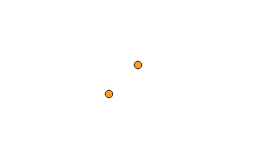
\includegraphics[width=12cm]{figures/1174008/2/hasilsoal1.PNG}
		\centering
		\caption{Point}
	\end{figure}
	
	\item 
	\lstinputlisting{src/1174008/2/Soal2.py}
	\begin{figure}[H]
		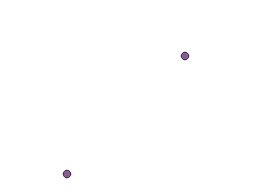
\includegraphics[width=12cm]{figures/1174008/2/hasilsoal2.PNG}
		\centering
		\caption{Point}
	\end{figure}
	
	\item 
	\lstinputlisting{src/1174008/2/Soal3.py}
	\begin{figure}[H]
		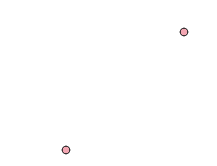
\includegraphics[width=12cm]{figures/1174008/2/hasilsoal3.PNG}
		\centering
		\caption{Point}
	\end{figure}
	
	\item 
	\lstinputlisting{src/1174008/2/Soal4.py}
	\begin{figure}[H]
		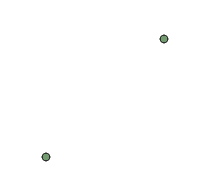
\includegraphics[width=12cm]{figures/1174008/2/hasilsoal4.PNG}
		\centering
		\caption{Point}
	\end{figure}
	
	\item 
	\lstinputlisting{src/1174008/2/Soal5.py}
	\begin{figure}[H]
		
\includegraphics[width=12cm]{figures/1174008/2/hasilsoal5.PNG}
		\centering
		\caption{Polyline}
	\end{figure}
	
	\item 
	\lstinputlisting{src/1174008/2/Soal6.py}
	\begin{figure}[H]
		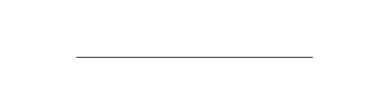
\includegraphics[width=12cm]{figures/1174008/2/hasilsoal6.PNG}
		\centering
		\caption{Poligon}
	\end{figure}
	
	\item 
	\lstinputlisting{src/1174008/2/Soal7.py}
	\begin{figure}[H]
		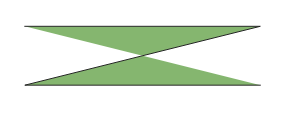
\includegraphics[width=12cm]{figures/1174008/2/hasilsoal7.PNG}
		\centering
		\caption{Polygon}
	\end{figure}
	
	\item 
	\lstinputlisting{src/1174008/2/Soal8.py}
	\begin{figure}[H]
		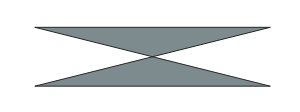
\includegraphics[width=12cm]{figures/1174008/2/hasilsoal8.PNG}
		\centering
		\caption{Polygon}
	\end{figure}
	
	\item 
	\lstinputlisting{src/1174008/2/Soal9.py}
	\begin{figure}[H]
		
\includegraphics[width=12cm]{figures/1174008/2/hasilsoal9.PNG}
		\centering
		\caption{Polygon}
	\end{figure}

    \item 
	\lstinputlisting{src/1174008/2/SoalMod.py}
	\begin{figure}[H]
		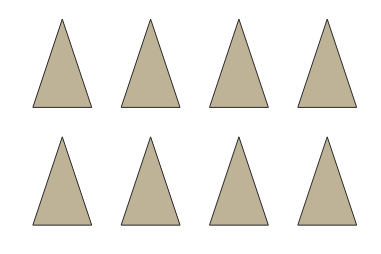
\includegraphics[width=12cm]{figures/1174008/2/hasilsoal10mod.PNG}
		\centering
		\caption{Hasil Mod saya 0 berberntuk segitiga sama kaki n = 8 jadi ada 8 buah}
	\end{figure}
\end{enumerate}

\subsection{Link}
\href{https://www.youtube.com/watch?v=Nd2ZXhCWFJU&t=6s}{Youtube}

\subsection{Plagiarism}
\begin{figure}[H]
	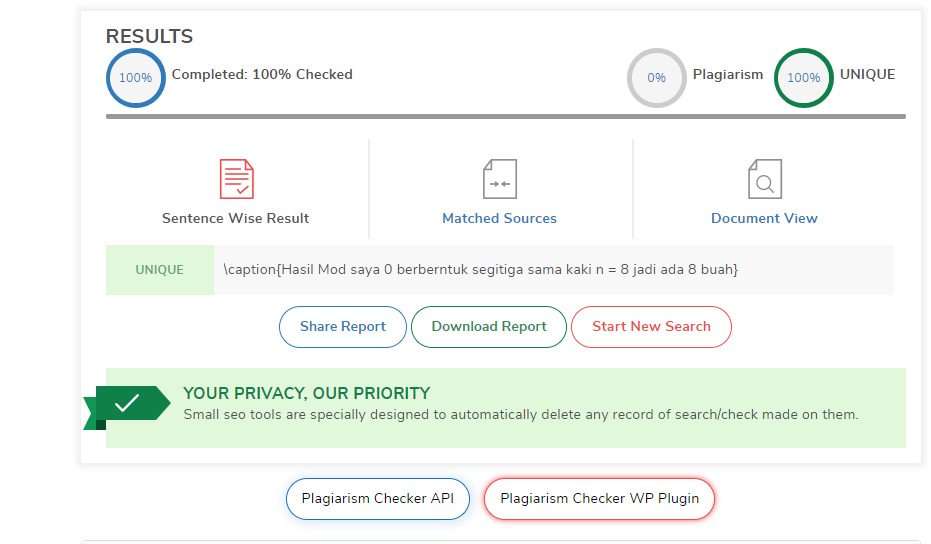
\includegraphics[width=4cm]{figures/1174008/2/hasilplagiat.PNG}
	\centering
	\caption{Bukti Tidak Melakukan Plagiat}
\end{figure}